% Included from both -slides and -handout versions.

\mode<presentation>
{
  \usetheme{default}
  \useoutertheme{infolines}
}

\usepackage[english]{babel}
\usepackage[latin1]{inputenc}
\usepackage{graphicx}
\usepackage{times}
\usepackage[T1]{fontenc}
\usepackage{fancyvrb}
\usepackage{hyperref}
\usepackage{listings}
\begin{document}
\lstset{language=C, escapeinside={(*@}{@*)}, numbers=left,
  basicstyle=\tiny, showspaces=false, showtabs=false}

\def\Tiny{\fontsize{4pt}{4pt} \selectfont}

\title{L41: Lab 5 - TCP Latency and Bandwidth}
\author{Dr Robert N. M. Watson}
\date{10 February 2016}

\begin{frame}
  \titlepage
\end{frame}

\section{Introduction}

\begin{frame}
  \frametitle{L41: Lab 5 - TCP latency and bandwidth}

  \begin{itemize}
    \item TCP congestion control
    \item TCP Protocol Control Block (TCPCB)
    \item Exploratory and experimental questions
  \end{itemize}
\end{frame}

\begin{frame}
  \frametitle{Lect 6: TCP goals and properties}

  \begin{columns}[T]
    \column{0.38\textwidth}
      \smallskip
      \begin{center}
	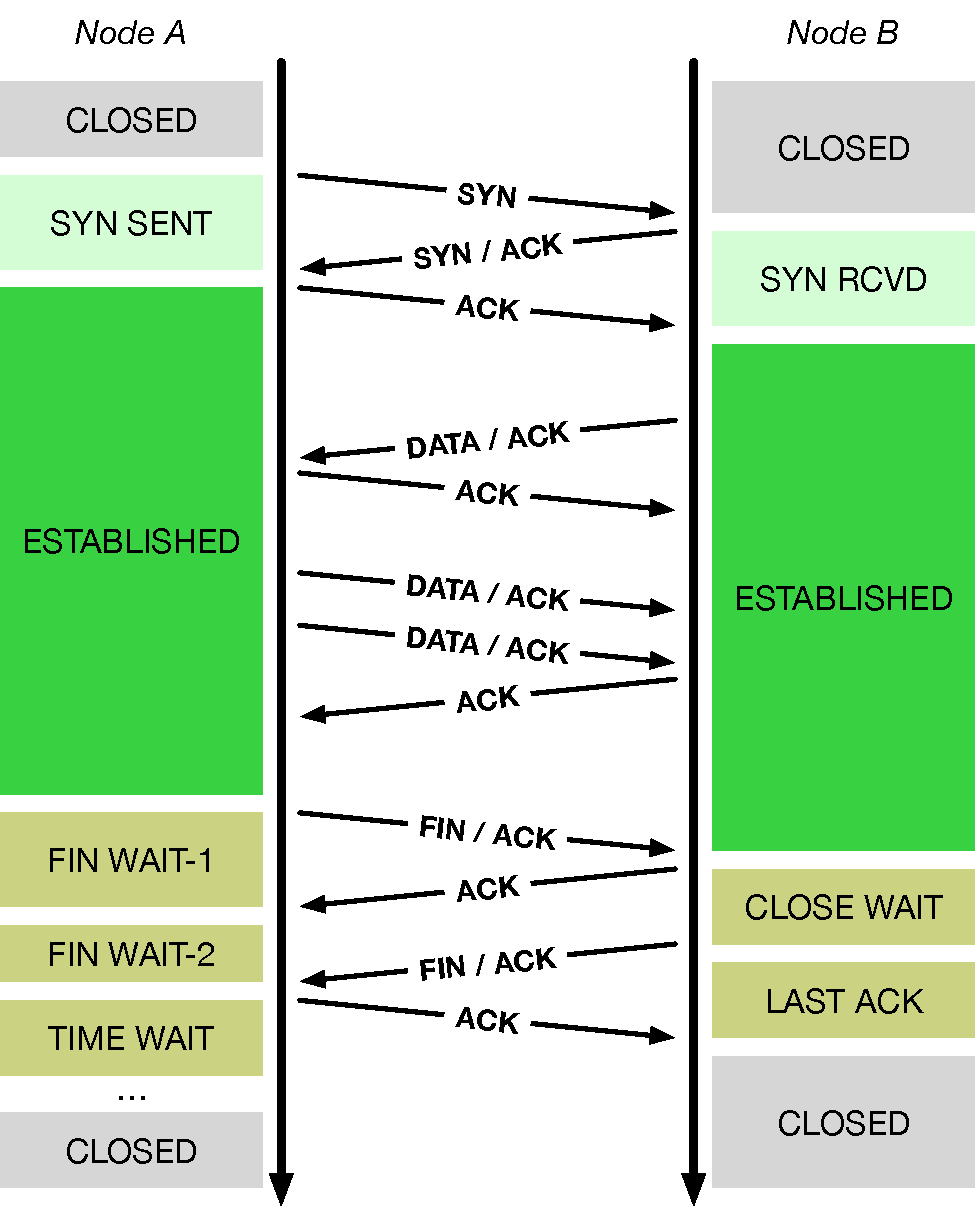
\includegraphics[width=1.15\textwidth]{../../figures/tcp-timeline.pdf}
      \end{center}

    \column{0.52\textwidth}

      \pause

      \begin{itemize}
	\item Network may delay, (reorder), drop, corrupt packets

	\pause

	\item TCP: Reliable, ordered, stream transport protocol over IP

	%\item Connections identified by unique IP-port 4-tuple

	\pause

	\item Three-way handshake: SYN~/ SYN-ACK~/ ACK (mostly!)

	\pause

	\item Sequence numbers ACK'd; data retransmitted on loss

	\pause

	\item Round-Trip Time (RTT) measured to time out loss

	\pause

        \item Flow control via advertised window size in ACKs

	\pause

	\item Congestion control (`fairness') via packet loss and ECN

	%\pause

	%\item Complex teardown permits `half-close' and port reuse
      \end{itemize}

  \end{columns}
\end{frame}

\begin{frame}
  \frametitle{Lect 6: TCP congestion control and avoidance}

  \begin{columns}[T]
    \column{0.35\textwidth}
      \begin{center}
	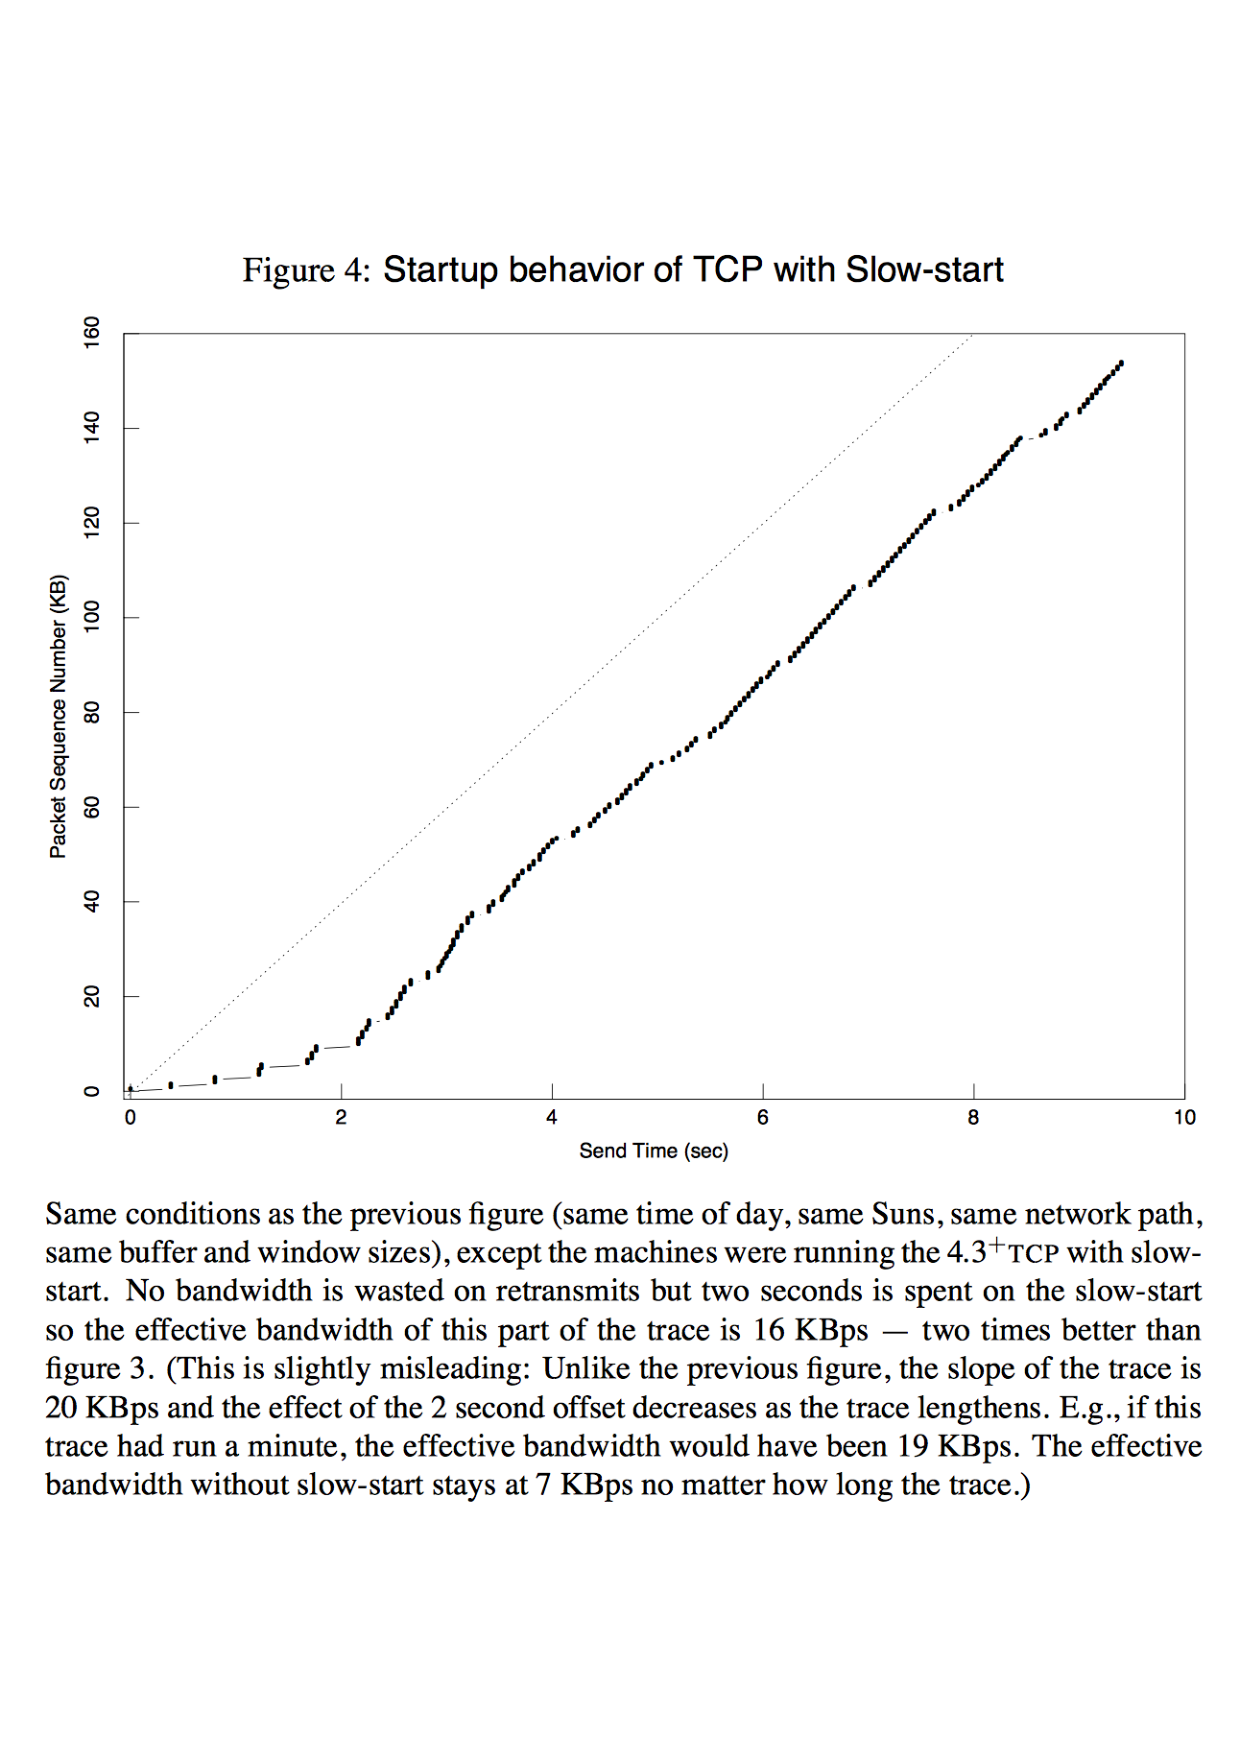
\includegraphics[width=1.2\textwidth]{../../figures/vj-congestion-slow-start.pdf}
      \end{center}

    \column{0.55\textwidth}

      \pause

      \begin{itemize}
	\item 1986 Internet CC collapse
	\begin{itemize}
	  \item 32Kbps -> \textbf{40bps}
	\end{itemize}

	\pause

	\item Van Jacobson, SIGCOMM 1988
	\begin{itemize}
	  \item Don't send more data than the network can handle!

	  \pause

	  \item \textbf{Conservation of packets} via ACK clocking

	  \pause

	  \item Exponential retransmit timer, slow start, aggressive receiver
	    ACK, and dynamic window sizing on congestion
        \end{itemize}

	\pause

        \item ECN (RFC 3168), ABC (RFC 3465), Compound (Tan, et al, INFOCOM
	  2006), Cubic (Rhee and Xu, ACM OSR 2008)
      \end{itemize}
  \end{columns}
\end{frame}

\begin{frame}
  \frametitle{Lect 6: TCP time/sequence graphs}

  \begin{columns}[T]
    \column{0.55\textwidth}
      \bigskip
      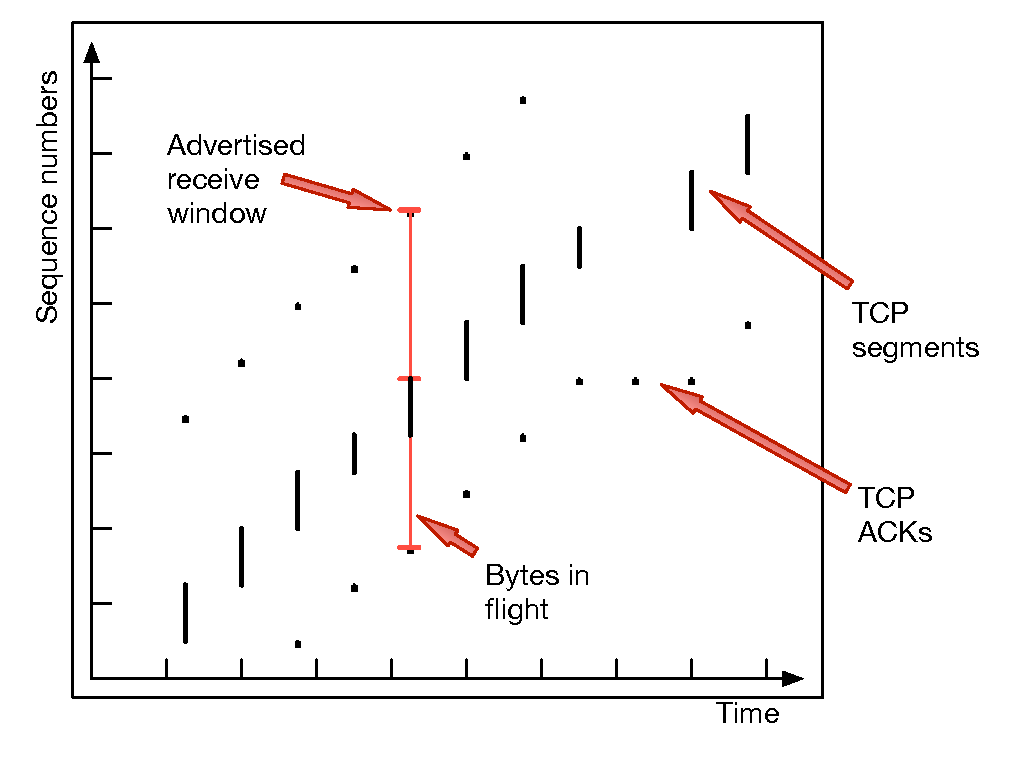
\includegraphics[width=1.2\textwidth]{../../figures/tcp-time-sequence.pdf}

    \column{0.35\textwidth}
    \begin{itemize}

      \bigskip
      \pause

      \item Extracted from TCP packet traces

      \medskip
      \pause

      \item Visualise windows, congestion response, RTT, etc.
      \begin{itemize}
	\item X: Time
	\item Y: Sequence number
      \end{itemize}

      \medskip
      \pause

      \item We can also extract this data from the stack using DTrace
    \end{itemize}
  \end{columns}
\end{frame}

\begin{frame}
  \frametitle{Lect 6: Data structures - sockets, control blocks}

  \begin{center}
    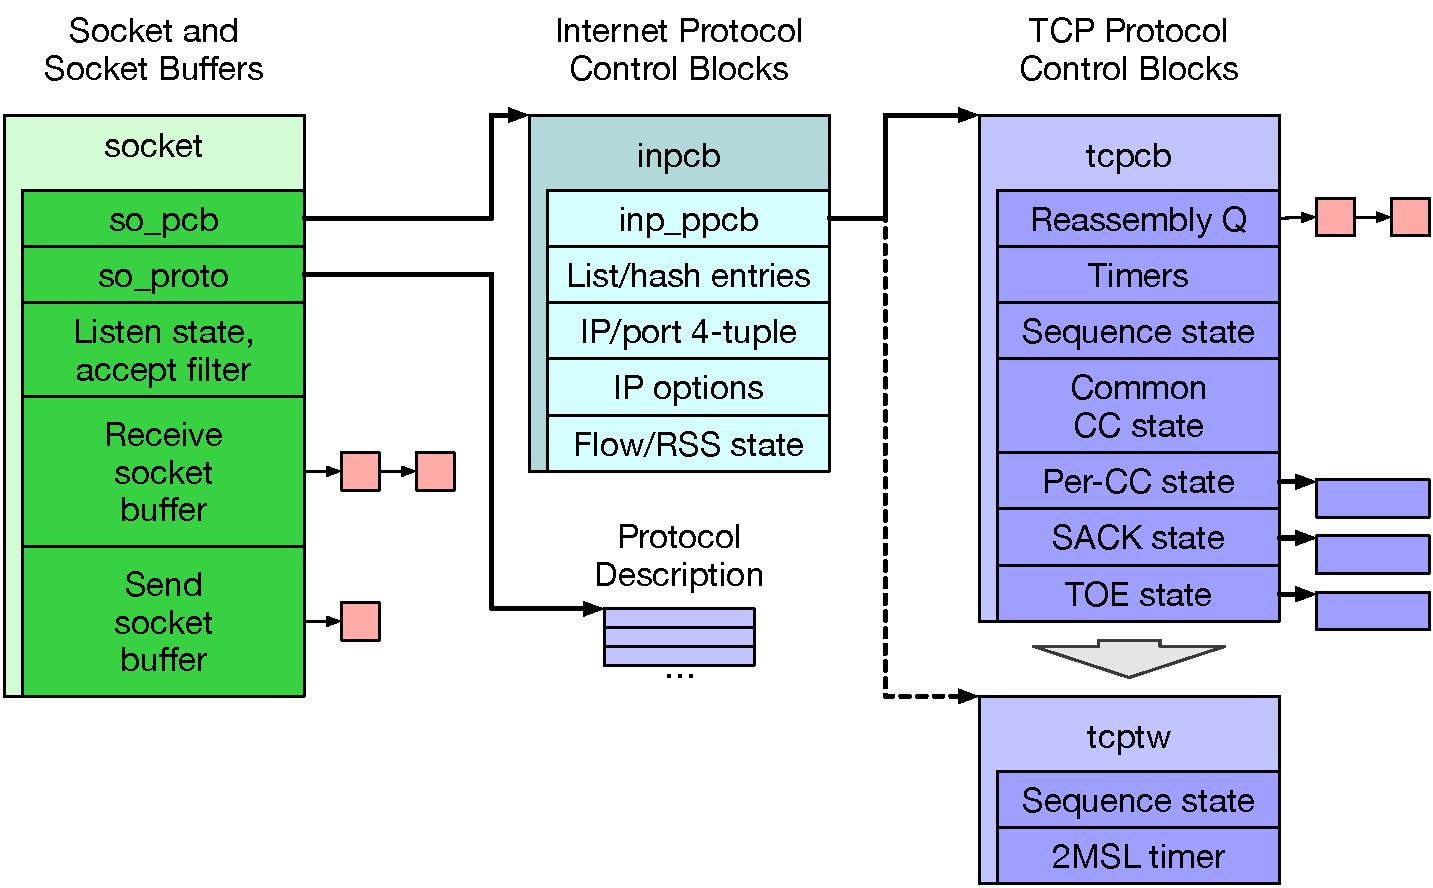
\includegraphics[width=\textwidth]{../../figures/tcp-structures.pdf}
  \end{center}
\end{frame}

\begin{frame}
  \frametitle{\texttt{tcpcb} sender-side data-structure fields}

  Described in more detail in the lab assignment:

  \medskip

  \begin{description}
    \item[\texttt{snd\_wnd}] Last received advertised flow-control window.
    \item[\texttt{snd\_cwnd}] Current calculated congestion-control window.
    \item[\texttt{snd\_ssthresh}] Current show-start threshold: if
      \texttt{snd\_cwnd} is less than or equal to \texttt{snd\_ssthresh}, then
      TCP is in slow start; otherwise, it is in congestion avoidance.
  \end{description}

  \medskip

  \begin{itemize}
    \item Instrument \texttt{tcp\_do\_segment} using DTrace to inspect TCP
      header fields and \texttt{tcpcb} state
    \item Packets on `client' and `server'; \texttt{tcpcb} only on `server'.
    \item Use as input to time--sequence-number or time--bandwidth plots.
    \item Make sure to flush the TCP host cache between benchmark runs.
  \end{itemize}
\end{frame}

\begin{frame}
  \frametitle{Exploratory questions}

  \begin{itemize}
    \item As latency varies, how does overall bandwidth change?
    \item How does using a fixed rather than auto-resized socket buffer affect
      advertised receive window?  Use a fixed buffer size (1MB).
    \item How quickly does TCP enter steady state (i.e., shift out of slow
      start) at a 10ms RTT?
      Is this a product of the congestion or the socket-buffer limit?
  \end{itemize}
\end{frame}

\begin{frame}
  \frametitle{Experimental questions for the lab report}

  \begin{itemize}
    \item Plot network latency vs. TCP bandwidth.
      Does linear increase in latency mean linear decrease in bandwidth?
      How does socket-buffer auto-resizing help/hurt/not change performance?
    \item Explore the effects of socket-buffer limits and stack graph
      information on the flow-control versus congestion-control limits.
      How does socket-buffer auto-resizing help/hurt/not change performance?
    \item Explore how latency affects the time taken to leave slow start.
  \end{itemize}
\end{frame}

\begin{frame}
  \frametitle{This lab session}

  \begin{itemize}
    \item Ensure that you are able to properly extract both TCP header and
      \texttt{tcpcb} fields from the \texttt{tcp\_do\_segment} FBT probe
    \item Generate the data for a time--bandwidth graph
    \item Generate the data for a time--sequence-number graph
    \item Ask us if you have any questions or need help
  \end{itemize}
\end{frame}

\end{document}
